\subsection{Auswertung}
Um das laufende Training und bereits abgeschlossene Trainingseinheiten zu bewerten oder zu vergleichen, nutzt Unity ML-Agents Tensorboard. Tensorboard visualisiert die Metriken des Trainings in Zeitgraphen (siehe Abbildung \ref{fig:tensorboard}). Der wichtigste Graph ist die gesammelte Belohnung, die ein Maß für den Erfolg des Agenten darstellt. Für Implementierungen mit frühem Stoppen, eine Technik für das frühe Beenden einer Trainingsepisode zur Vermeidung von Training in unvorteilhaften Zuständen, ist die erreichte Episodenlänge ebenfalls sehr aussagekräftig, da sie anzeigt, wie lange der Agent in der Umgebung bestehen kann. Unter der Rubrik \grqq{}Policy\grqq{} finden sich auch die Graphen, welche den Verlauf der Hyperparameter darstellen. Die linke Seitenleiste listet alle im aktuellen Verzeichnis gespeicherten Trainingseinheiten auf. Darüber können Trainingsets ausgewählt und anschließend in den Graphen durch unterschiedlich farbige Linien verglichen werden. Diese Visualisierungen ermöglichen eine detaillierte Analyse und den Vergleich verschiedener Trainingsläufe, was zur Optimierung des Trainingsprozesses beiträgt.

\begin{figure}[H]
  \centering  
  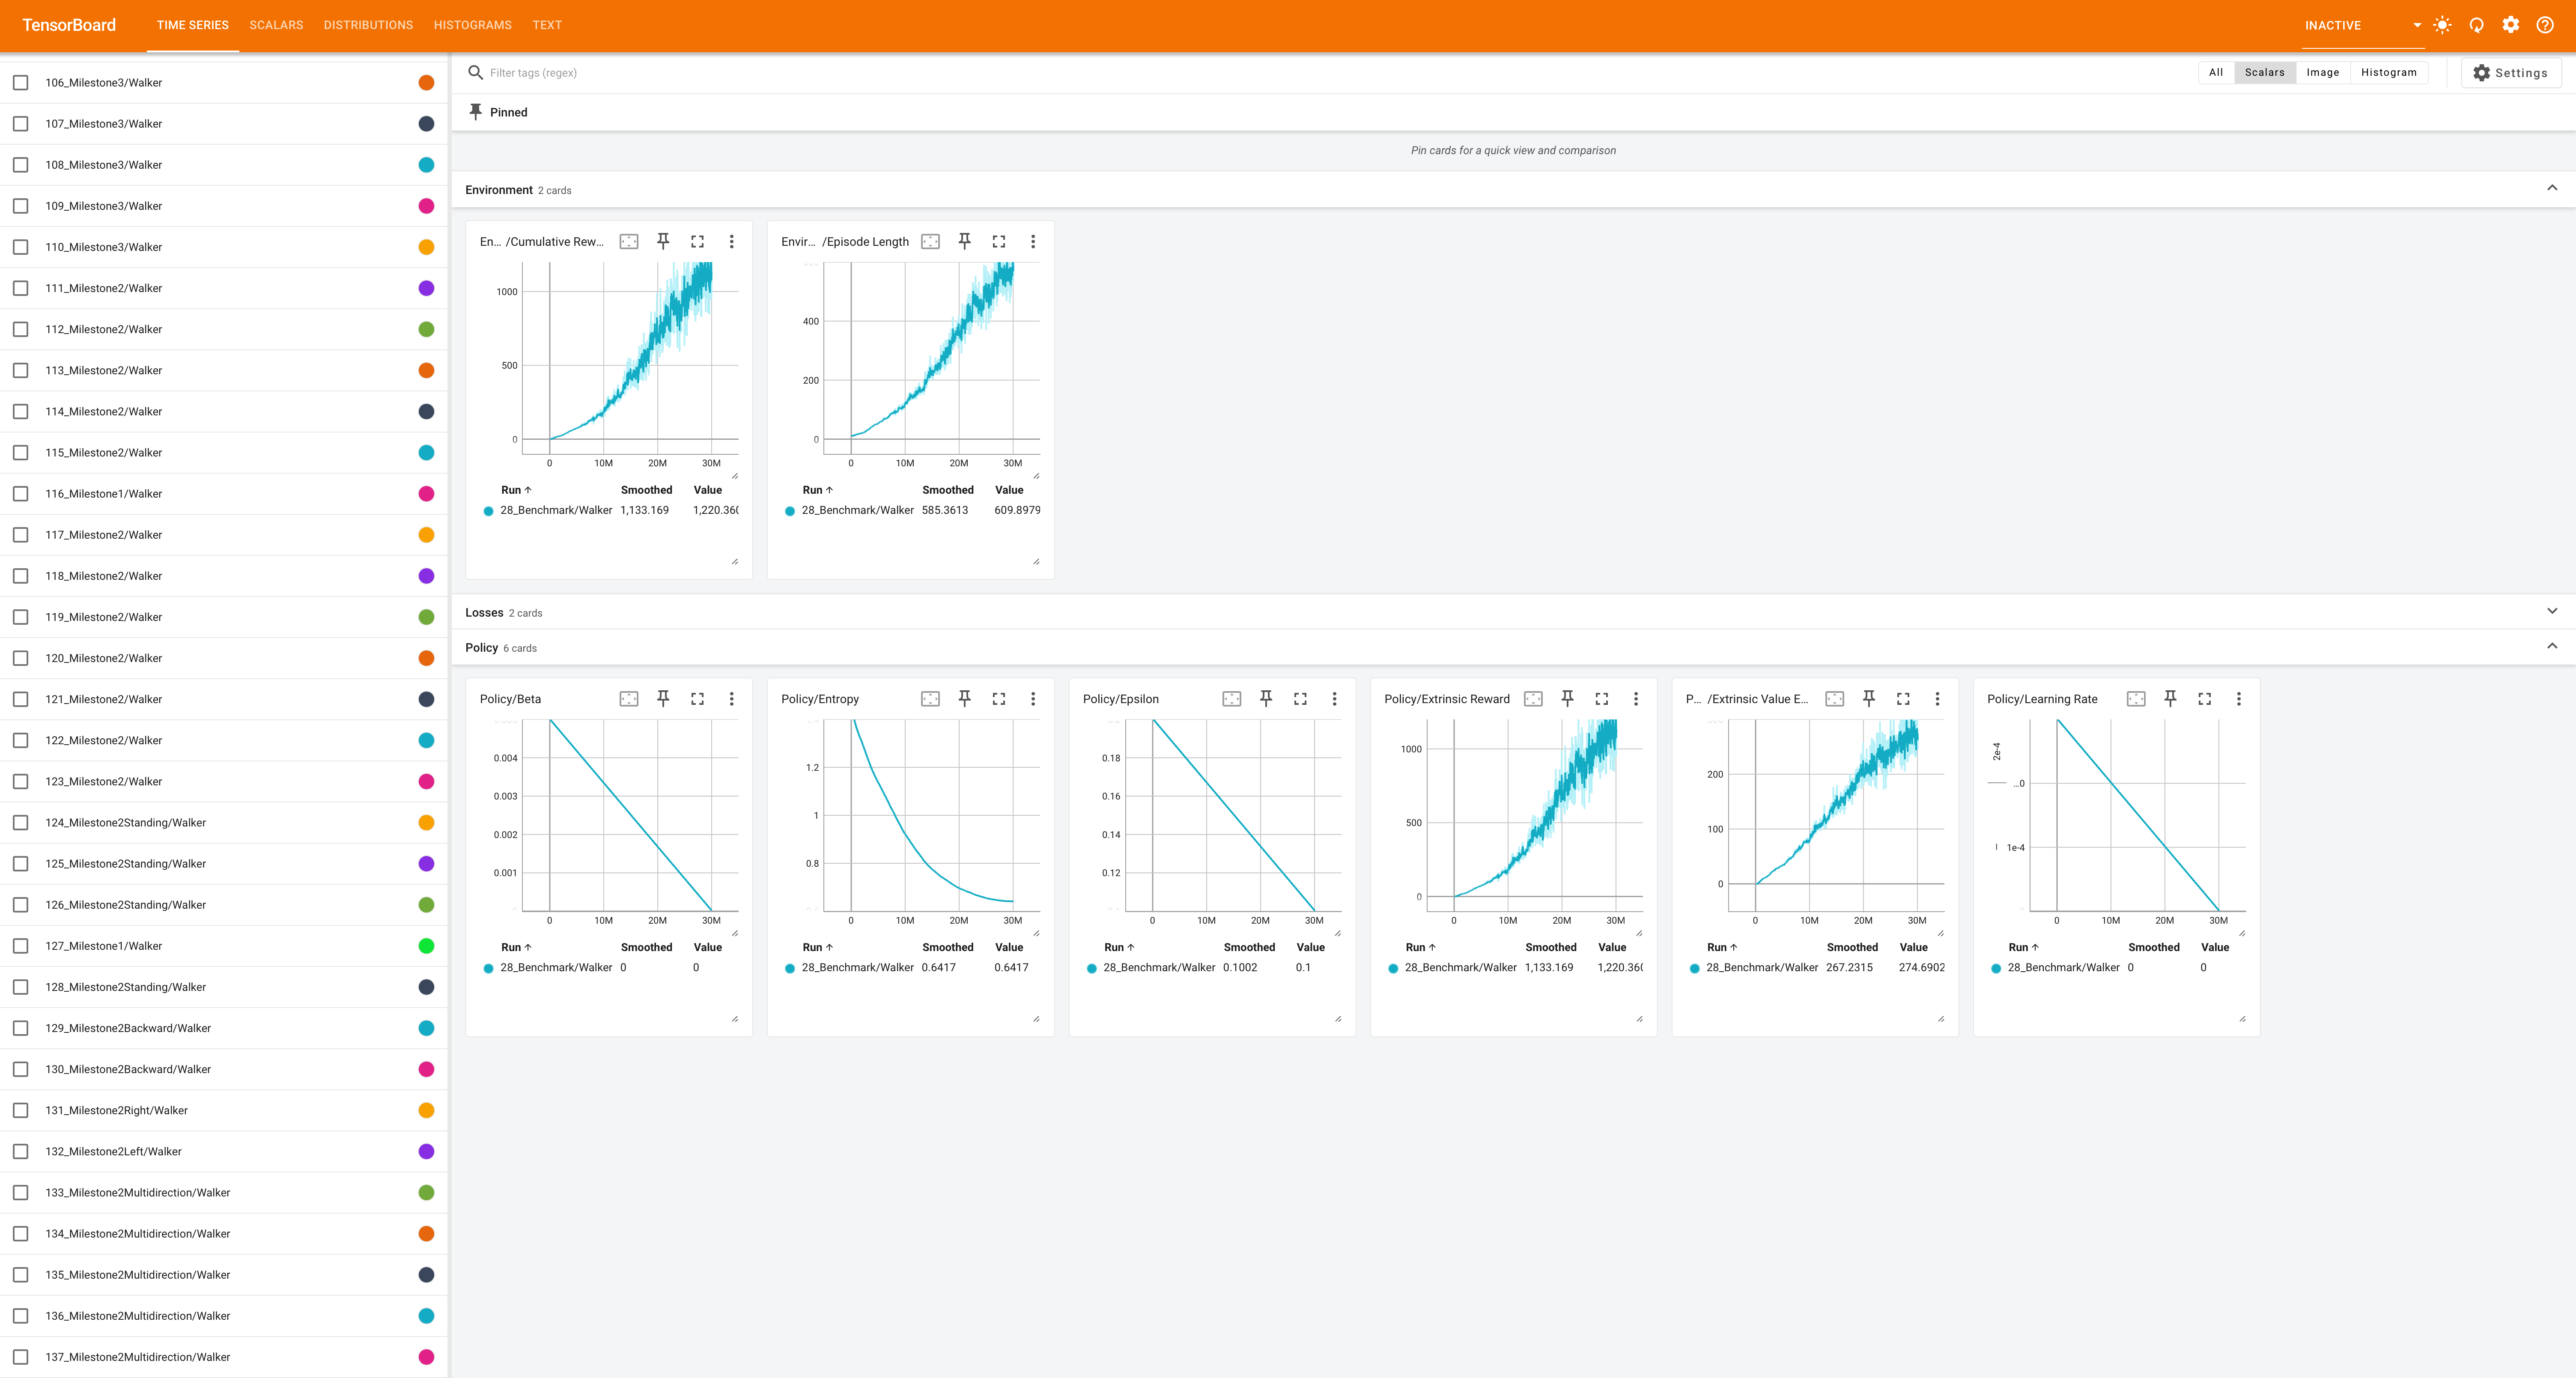
\includegraphics[width=0.9\textwidth]{img/tensorboard}
  \caption{Tensorboard Ansicht}
  \label{fig:tensorboard}
\end{figure}

Nicht immer geben die vorgefertigten Graphen alle relevanten Informationen wieder. Um die erfassten Daten und damit die Graphen zu erweitern, bietet Unity ML-Agents über die Statistikrekorder die \grqq{}Statistik Hinzufügen\grqq{} Funktion. Neu hinzugefügte Werte werden über die Episode und alle Umgebungen aggregiert. Als Aggregationsmethode kann zwischen Duchschnitt und letztem Wert entschieden werden. In Tensorboard werden die neuen Statistiken anschließend dargestellt.

Die letzte Instanz der Auswertung ist das Abspielen des trainierten Modells in der Unity-Umgebung. In den meisten Fällen ist die grafische Darstellung das zuverlässigste Medium, um das trainierte Modell zu bewerten, da sie ermöglicht, das Verhalten des Agenten in Echtzeit und in seiner tatsächlichen Umgebung zu beobachten. Dies bietet wertvolle Einblicke in die Effektivität und Robustheit des Modells, die durch numerische Metriken allein nicht erfasst werden können.